\cleardoublepage  
\chapter{Methodology}
\label{chap:methodology}

\section{Development Methodology}
\label{sec:devmet}

\section{Solution Design Methodology}
\label{sec:solmet}

\subsection{Description}

similarity measures of Vetkamp has a nice explanation 
of how to approach shape matching.

\subsection{Thresholding}
\label{sec:metthres}

Since the main purpose of this study is to fit the shape of \emph{C.Elegans} worms on digital
images, it is useful to differentiate these from the rest of the image in order to perform a more 
accurate analysis. The shape of the worms
can be characterized as objects and the rest of the image as background. More precisely
the image pixels can be separated into two groups: object pixels, that are all of those
that belong to a worm shape and background pixels, that are all the remaining ones.\\

Given this theoretical characterization, a thresholding filter would come to be a useful tool 
to locate the objects of study in the digital representation and to discard unnecessary 
information, obtaining a binary image from the original one. A binary image would then provide
an initial segmentation of the processed image, being as well a key element to obtain
a distance transformation, as it is explained in Sec. \ref{sec:metdt}.

\subsubsection{Implementation}
There are four thresholding filters for 2D images implemented on \emph{Endrov}, these are: 
\emph{Fukunaga},\emph{Max entropy}, \emph{Otsu} and \emph{Percentile}, that cover the 
histogram and entropy-based thresholding methods categories as defined in Sec.\ref{sec:thresholding}.
Considering that the implemented methods are sufficiently different and given the transparency
of \emph{C.Elegans} worms is hard to determine theoretically which would be the most appropriate 
thresholding method to obtain an accurate binary image, from the study data-set. In order 
to select a thresholding method a series of experiments where performed tweaking the parameters
for the different mentioned methods, as it is explained on Sec.\ref{exp:thres}.
The selected method was \emph{Percentile Threshold 2D} with a percentile value oscilating from
$0.072$ to $0.09$ on the different test images.\\

Figure \ref{fig:wormthres} shows a binary image obtained after applying
the \emph{Percentile Threshold 2D} method with a percentile value of $0.074$

\begin{figure}
  \centering
  \subfloat[Original image]{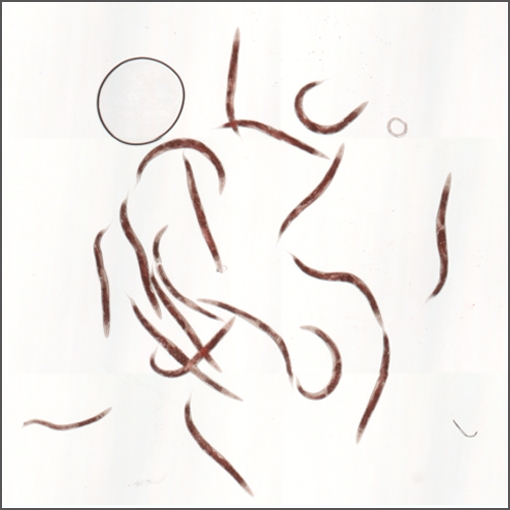
\includegraphics[width=0.45\textwidth]{original.png}}
\qquad
  \subfloat[Percentil Threshold. Value=0.074]{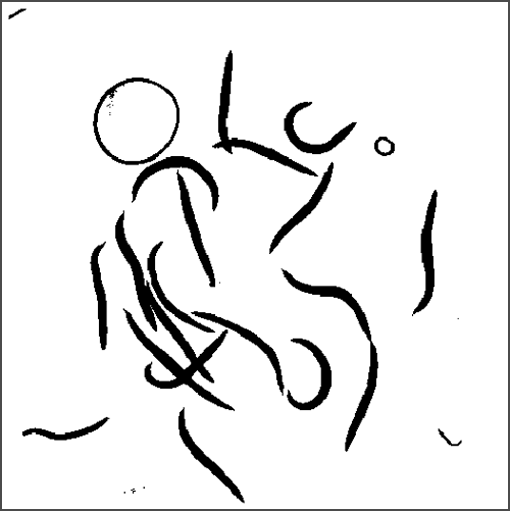
\includegraphics[width=0.45\textwidth]{thres/worms}}
\caption{Worms in liquid media original image and binary image obtained through
Percentile Thresholding with a percentile value of 0.074}
  \label{fig:wormthres}
\end{figure}

\subsection{Distance transformation}
\label{sec:metdt}

In this shape fitting approach for \emph{C.Elegans} worms the distance transformation
of the given image is used thoroughly for contour detection and different kinds of image 
segmentation procedures. Specifically the distance map allows to detect and follow
the exact contour of isolated worms (Sec. \ref{sec:metiso}), 
is useful in the shape profile generation (Sec. \ref{sec:metwormprof}), and essential in the heuristical
guessing of the more likely worm-paths on \emph{worm clusters} (Sec. \ref{sec:metcluster}).
It also improves the performance of the iterative thinning algorithm designed by 
\emph{Zhang and Suen} \cite{thinning} as it is described on Sec.\ref{sec:metsk}

\subsubsection{Implementation}
\label{sec:dtimp}

 As stated in \cite[p.196]{fastdt} the algorithms of DT can be categorized into two classes: one is the iterative 
 method which is efficient in a cellular array computer since all the pixels at each iteration can be processed in parallel, and the other 
is sequential (or recursive) method which is suited for a conventional computer by
 avoiding iterations with the efficiency to be independent of object size. 
Using the general machines that most people working in digital image processing
 have access to, sequential algorithms are often much more efficient than
 iterative ones. For this reason a sequential approach was chosen to calculate the
distance transformation of the input images. Particularly the two-scans transformation
using 3x3 neighborhoods \cite{fastdt} which is both efficient and easy to implement.\\

In the mentioned paper a distance map calculation algorithm is described which consist
on only two scans of the image bitmap, one left to right - top to bottom, and another
right to left - bottom to top, with one operation per pixel. This makes the complexity
of the algorithm $\mathcal{O}(N)$ for $N$ the size of the image array.
In \cite[p.197]{fastdt} a pseudo-code for \emph{Chessboard} and 
\emph{Manhattan or city-block} distances is given, while in \cite[p.198]{fastdt} the 
definition is extended to improve the efficiency of the calculations needed to 
generate a distance map using \emph{Euclidean} distances.
The two-scans algorithm was implemented using the three different distance metrics
mentioned before. This allows a wider analysis on the behavior and accuracy of the shape 
fitting process from one metric to another.``The city block or chessboard distance
measures are sensitive to the rotations of an object, but the Eculidean distance
measure is rotation invariant. However, its square root operation is costly...''
\cite[p.332]{eucskeleton}. Given the strait shape of worms and the different levels
of accuracy of the distance metrics it is hard to tell at first sight which would be 
the most adequate to use.
The figure \ref{fig:distance} shows the binary image three and the distance maps obtained 
from a single worm image.

\begin{figure}
  \centering
  \subfloat[Binary Image]{\label{fig:manh}
\includegraphics[width=0.45\textwidth]{dt/binary}}
\qquad
  \subfloat[Manhattan metric]{\label{fig:manh}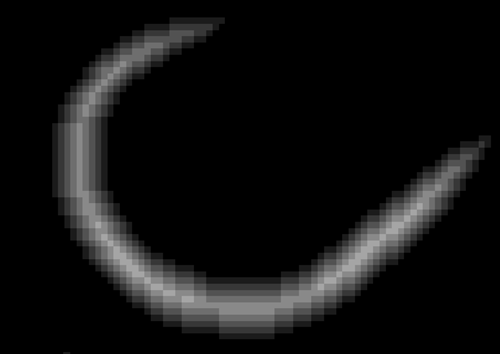
\includegraphics[width=0.45\textwidth]{dt/manhattandt}}
\qquad                
  \subfloat[Chessboard metric]{\label{fig:chess}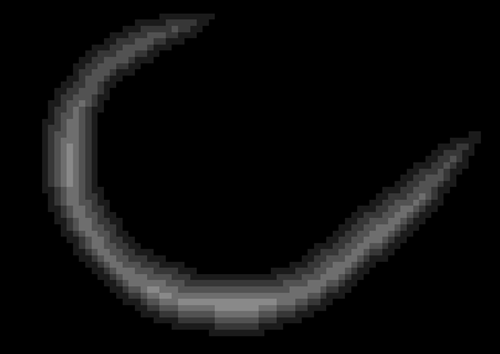
\includegraphics[width=0.45\textwidth]{dt/chessboarddt}}
\qquad
  \subfloat[Euclidean metric]{\label{fig:mouse}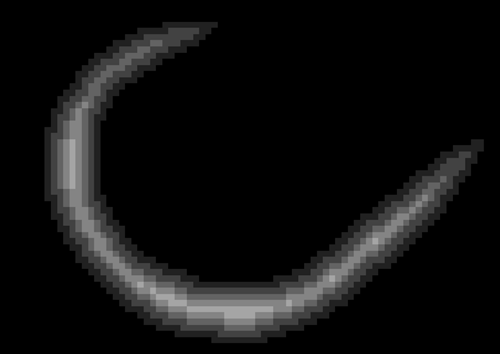
\includegraphics[width=0.45\textwidth]{dt/euclideandt}}
  \caption{Binary Image and Three Distance Transformation metrics from a single worm image}
  \label{fig:distance}
\end{figure}


\subsection{Worm Skeletonization}
\label{sec:metsk}

\subsection{Worm Segmentation}
\label{sec:metcluster}

\subsubsection{Clustering}
\label{sec:metcluster}
\subsubsection{Path guessing}

\subsection{Worm Shape Descriptor}
\label{sec:metshapedescriptor}

\subsubsection{Worm Profile Generation}
\label{sec:metwormprof}

\subsection{Triangle mesh and rasterization}
\label{sec:metrast}

\subsection{Profile-driven shape fitting}
\label{sec:metfit}

Check b-splines snakes.. Talks about avoding internal energy

\subsubsection{Worm Cluster shape fitting}
\subsubsection{Isolated Worms shape fitting}
\label{sec:metiso}